\documentclass[aspectratio=169,10pt]{beamer}

\usetheme{metropolis}
\metroset{sectionpage=none}
\usepackage{fontspec}
\usepackage{booktabs}
\usepackage{tabularx}
\usepackage{fontawesome5}
\usepackage{tikz}
\usetikzlibrary{arrows.meta,positioning}

\definecolor{accent}{HTML}{0F6E6E}
\definecolor{muted}{HTML}{6B7280}
\definecolor{soft}{HTML}{E6F2F2}

\setbeamercolor{palette primary}{bg=accent, fg=white}
\setbeamercolor{frametitle}{bg=accent, fg=white}
\setbeamercolor{progress bar}{fg=accent, bg=accent!25}
\setbeamercolor{alerted text}{fg=accent}
\setbeamercolor{block title}{bg=accent!15, fg=accent}
\setbeamercolor{block body}{bg=soft, fg=black}

\setbeamertemplate{itemize items}[circle]
\setbeamertemplate{caption}{\raggedright\insertcaption\par}

\newcommand{\code}[1]{\texttt{\small #1}}

\tikzset{
  box/.style={draw=accent, fill=soft, rounded corners=2pt, align=center,
              font=\footnotesize, inner sep=4pt, minimum height=8mm},
  flow/.style={-{Latex[length=2mm]}, accent!70, thick}
}

\begin{document}

\begin{frame}[plain,noframenumbering]
  \vfill
  {\usebeamerfont{title}\color{accent}\Huge Kodebasen\\[0.15em] i overblik\par}
  \vspace{0.4em}
  {\usebeamerfont{subtitle}\color{muted}\Large Bumle Business -- VPN-logovervågning\par}
  \vspace{1.4em}
  \textcolor{accent}{\rule{4cm}{2pt}}
  \vfill
  {\small Python 3.10+ \quad$\cdot$\quad Standardbibliotek, Dash og Plotly\par}
\end{frame}

\begin{frame}{Dagsorden}
  \begin{columns}[T]
    \column{0.48\textwidth}
    \begin{itemize}
      \item Opgaven og løsningens formål
      \item Dataflow fra rå log til indsigt
      \item Arkitektur og ansvarsdeling
      \item Analyse, detektion og visualisering
      \item Kodekvalitet, tests og dokumentation
    \end{itemize}
    \column{0.46\textwidth}
    \begin{block}{Fokus}
      \small Overblik og sammenhænge.\\
      Implementeringsdetaljer vises kun, hvor de forklarer en grænseflade.
    \end{block}
  \end{columns}
\end{frame}

\begin{frame}{Opgaven}
  \begin{columns}[T]
    \column{0.54\textwidth}
    Bumle Business har mistanke om uautoriseret adgang via VPN.
    \vspace{0.6em}
    \begin{itemize}
      \item Rå loglinjer er svære at læse og sammenligne
      \item Mistænkelig aktivitet skal kunne findes uden at læse filen igennem
      \item Løsningen skal vise både enkeltposter og mønstre
    \end{itemize}
    \column{0.42\textwidth}
    \begin{block}{Løsningen}
      \small Loggen indlæses i hukommelsen, parses til records og præsenteres i konsoltabeller og et interaktivt dashboard med diagrammer og detektion.
    \end{block}
  \end{columns}
  \vfill
  {\footnotesize\color{muted}\code{cyber\_security\_log\_sample.txt} -- 541 linjer, 9 faste kolonner.}
\end{frame}

\begin{frame}{Dataflow}
  \begin{center}
    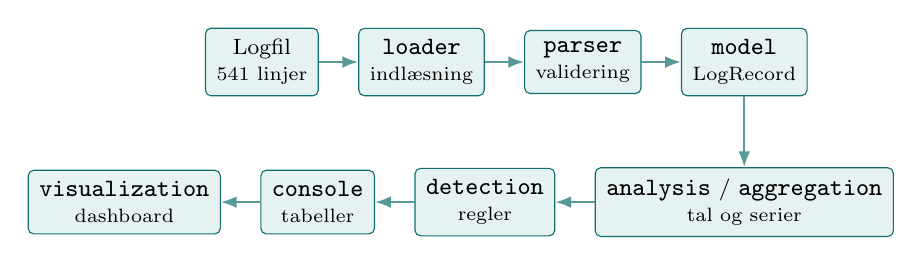
\begin{tikzpicture}[node distance=4mm and 5mm]
      \node[box] (file) {Logfil\\{\scriptsize 541 linjer}};
      \node[box, right=of file] (loader) {\code{loader}\\{\scriptsize indlæsning}};
      \node[box, right=of loader] (parser) {\code{parser}\\{\scriptsize validering}};
      \node[box, right=of parser] (model) {\code{model}\\{\scriptsize LogRecord}};
      \node[box, below=9mm of model] (analysis) {\code{analysis} / \code{aggregation}\\{\scriptsize tal og serier}};
      \node[box, left=of analysis] (detect) {\code{detection}\\{\scriptsize regler}};
      \node[box, left=of detect] (console) {\code{console}\\{\scriptsize tabeller}};
      \node[box, left=of console] (viz) {\code{visualization}\\{\scriptsize dashboard}};

      \draw[flow] (file) -- (loader);
      \draw[flow] (loader) -- (parser);
      \draw[flow] (parser) -- (model);
      \draw[flow] (model) -- (analysis);
      \draw[flow] (analysis) -- (detect);
      \draw[flow] (detect) -- (console);
      \draw[flow] (console) -- (viz);
    \end{tikzpicture}
  \end{center}
  \vspace{0.4em}
  \begin{columns}[T]
    \column{0.32\textwidth}
    {\footnotesize\textbf{Ind } \\\scriptsize Fil $\rightarrow$ tekstlinjer $\rightarrow$ \code{LogRecord}}
    \column{0.32\textwidth}
    {\footnotesize\textbf{Beregn } \\\scriptsize Funktioner returnerer data, de printer ikke}
    \column{0.32\textwidth}
    {\footnotesize\textbf{Vis } \\\scriptsize Samme data bruges af CLI og dashboard}
  \end{columns}
\end{frame}

\begin{frame}{Arkitektur}
  \centering
  \small
  \begin{tabularx}{\textwidth}{@{}l X@{}}
    \toprule
    \textbf{Mappe} & \textbf{Ansvar} \\
    \midrule
    rod            & \code{config}, \code{errors}, \code{model}, \code{parser}, \code{loader}, \code{analysis}, \code{main} \\
    \code{aggregation}  & Gruppering og optælling pr. bruger, IP, vært og port \\
    \code{detection}    & Regelbaseret flagning af mistænkelige konti \\
    \code{console}      & Konsoltabeller over de grupperede rækker \\
    \code{visualization}& Dashboard, fire diagrammer, Plotly-tabeller og logfilter \\
    \code{tests}        & Tests og loguddrag til parser, model og loader \\
    \bottomrule
  \end{tabularx}
  \vfill
  {\footnotesize\color{muted}Én opgave pr. modul: indlæsning kender ikke til diagrammer, og analysen kender ikke til Dash.}
\end{frame}

\begin{frame}{Datagrundlaget}
  \begin{columns}[T]
    \column{0.50\textwidth}
      \textbf{Ni faste kolonner}
      \vspace{0.3em}
      \begin{itemize}
        \item \code{timestamp}, \code{level}, \code{event}
        \item \code{user}, \code{src\_ip}
        \item \code{dest\_host}, \code{dest\_port}
        \item \code{status}, \code{msg}
      \end{itemize}
      \vspace{0.3em}
      {\footnotesize\color{muted}Kolonnebredder og feltnavne ligger samlet i \code{config.py}.}
    \column{0.46\textwidth}
      \textbf{Berigelse i \code{model.py}}
      \vspace{0.3em}
      \begin{itemize}
        \item \code{classify\_ip} -- intern eller ekstern
        \item \code{service\_name} -- port til servicenavn
        \item \code{categorize\_event}
        \item \code{categorize\_status}
      \end{itemize}
  \end{columns}
  \vspace{0.6em}
  \begin{block}{Robusthed}
    \small Ugyldige linjer afvises med en \code{ParseError} og samles i en fejlliste, så resten af loggen stadig indlæses.
  \end{block}
\end{frame}

\begin{frame}{Analyse og aggregering}
  \begin{columns}[T]
    \column{0.48\textwidth}
      \textbf{\code{aggregation/}}
      \vspace{0.3em}
      \begin{itemize}
        \item \code{grouped\_rows} -- fælles grundlag for top-10
        \item \code{count\_by\_field} -- level, event, status, bruger
        \item \code{get\_user\_ip\_summary} -- unikke IP'er pr. bruger
      \end{itemize}
    \column{0.48\textwidth}
      \textbf{\code{analysis.py}}
      \vspace{0.3em}
      \begin{itemize}
        \item Top-10 brugere, kilde-IP'er og værter
        \item Fejlrate pr. bruger og pr. port
        \item Events pr. time og periodeafgrænsning
      \end{itemize}
  \end{columns}
  \vfill
  {\footnotesize\color{muted}Funktionerne tager records ind og returnerer lister og dictionaries -- ingen print, ingen Plotly. Derfor kan både CLI, dashboard og plots genbruge dem.}
\end{frame}

\begin{frame}{Detektion af mistænkelige konti}
  \begin{columns}[T]
    \column{0.52\textwidth}
      \textbf{Regelbaseret tælling pr. bruger}
      \vspace{0.3em}
      \begin{itemize}
        \item \code{ALERT} -- 4 forekomster
        \item \code{MALWARE\_SIGNATURE\_MATCH} -- 2 forekomster
        \item Tærsklerne ligger i \code{SUS\_DETECTION}
        \item Hver regel valideres ved opstart
      \end{itemize}
    \column{0.44\textwidth}
      \begin{block}{Fundet}
        \small Walter er det første brud: mange fejlede logins, derefter et vellykket login. Sporet fører til IP'en 172.16.0.44, et malware-match og til sidst et reset af admin-password.
      \end{block}
  \end{columns}
  \vspace{0.4em}
  {\footnotesize\color{muted}Login-forsøg er ikke en detektionsregel, men indgår i fejlraten, som vises i tabellerne og i dashboardet.}
\end{frame}

\begin{frame}{Visualisering}
  \begin{columns}[T]
    \column{0.46\textwidth}
      \textbf{Fem faner i dashboardet}
      \vspace{0.3em}
      \begin{itemize}
        \item Logtabel -- filtrering og sortering
        \item Overblik -- periode, fejlrate, unikke brugere og IP'er
        \item Diagrammer -- de fire plots
        \item Fejlandel pr. port
        \item Top 10 -- brugere, IP'er, værter
      \end{itemize}
    \column{0.50\textwidth}
      \textbf{Fire diagrammer}
      \vspace{0.3em}
      \begin{itemize}
        \item Time vs. antal events (scatter)
        \item Bruger vs. fejlrate (scatter med referencelinje)
        \item Port vs. eventtype (bobleplot: antal og IP-klasse)
        \item Eventtype vs. antal (søjler)
      \end{itemize}
  \end{columns}
  \vfill
  {\footnotesize\color{muted}\code{scatter\_plots.build\_figures} og \code{bar\_chart.event\_bar\_chart} bygger figurerne; \code{dashboard.create\_app} samler dem.}
\end{frame}

\begin{frame}{Grænseflader og genbrug}
  \centering
  \small
  \begin{tabularx}{\textwidth}{@{}l X@{}}
    \toprule
    \textbf{Grænseflade} & \textbf{Rolle} \\
    \midrule
    \code{load\_log\_file}        & Fil til tekstlinjer, med \code{LogFileError} ved problemer \\
    \code{log\_line\_parser}      & Linjer til records plus liste af afviste linjer \\
    \code{LogRecord}              & Fælles datamodel for alle lag \\
    \code{build\_view}            & Filtrering og sortering af logtabellen \\
    \code{track\_suspicious\_accounts} & Fund som tekst til terminalen \\
    \code{create\_app} / \code{run}    & Dashboard som Dash-app \\
    \bottomrule
  \end{tabularx}
  \vfill
  {\footnotesize\color{muted}Hvert lag kan testes og bruges uden at starte de øvrige.}
\end{frame}

\begin{frame}{Kodekvalitet}
  \begin{columns}[T]
    \column{0.48\textwidth}
      \textbf{Fejlhåndtering}
      \vspace{0.3em}
      \begin{itemize}
        \item \code{BumleBusinessError} som fælles base
        \item \code{LogFileError}, \code{ParseError}
        \item \code{DataError}, \code{DashboardError}
        \item Fejl oversættes til en pæn besked, ikke et crash
      \end{itemize}
    \column{0.48\textwidth}
      \textbf{Tests}
      \vspace{0.3em}
      \begin{itemize}
        \item Parser, model og loader
        \item Fixtures: gyldigt udsnit og grænsetilfælde
        \item \code{pytest} eller \code{main.py --run-tests}
        \item Coverage via \code{--coverage}
      \end{itemize}
  \end{columns}
\end{frame}

\begin{frame}[fragile]{Kørsel}
  \begin{columns}[T]
    \column{0.52\textwidth}
\begin{verbatim}
pip install -r requirements.txt
python main.py
python main.py --dashboard
\end{verbatim}
      \vspace{0.4em}
      {\footnotesize\color{muted}Dashboardet åbner på \\\code{http://127.0.0.1:8050}.}
    \column{0.44\textwidth}
      \textbf{Flag}
      \vspace{0.3em}
      \begin{itemize}
        \item \code{--log-file STI}
        \item \code{--dashboard}
        \item \code{--port PORT}
        \item \code{--run-tests}
        \item \code{--coverage}
      \end{itemize}
  \end{columns}
\end{frame}

\begin{frame}{Sammenfatning}
  \begin{columns}[T]
    \column{0.48\textwidth}
      \textbf{Styrker}
      \vspace{0.3em}
      \begin{itemize}
        \item Klar opdeling i indlæsning, analyse og præsentation
        \item Genbrugelige funktioner uden skjulte sideeffekter
        \item Regelbaseret detektion med konfigurerbare tærskler
      \end{itemize}
    \column{0.48\textwidth}
      \textbf{Næste skridt}
      \vspace{0.3em}
      \begin{itemize}
        \item Udvid testdækningen til analyse og visualisering
        \item Flere detektionsregler og korrelation på tværs af brugere
        \item Eksport af fund til en rapport
      \end{itemize}
  \end{columns}
  \vfill
  \begin{center}
    {\color{accent}\rule{4cm}{1.5pt}}\\[0.4em]
    {\footnotesize\color{muted}Fra 541 rå loglinjer til et overblik, der kan handles på.}
  \end{center}
\end{frame}

\end{document}
